\chapter{Plano Operacional}

\section{Arranjo físico}
Para exigir o menor investimento inicial possível, a empresa exercerá suas atividades em um escritório comercial com capacidade apenas para seus quatro sócios trabalharem e um pequeno espaço para o arquivamento dos documentos que não possam ser armazenados em meio digital. Este espaço estará disposto da seguinte como visto na figura \ref{fig:escritorio} abaixo.

\begin{figure}[!h]
  \begin{center}
    \frame{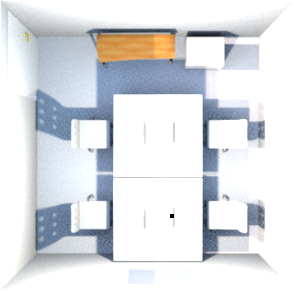
\includegraphics[width=70mm, height=60mm]{images/escritorio-frete-facil.png}}
    \caption{Vista superior da disposição do espaço de trabalho}
    \label{fig:escritorio}
  \end{center}
\end{figure}

Para tanto, o escritório será composto de 4 mesas para computador, 4 cadeiras, um arquivo e uma mesa de lado, totalizando um área útil mínima de $10m^{2}$.
